\documentclass[conference]{IEEEtran}
\usepackage{cite}
\usepackage{amsmath,amssymb,amsfonts}
\usepackage{algorithmic}
\usepackage{graphicx}
\usepackage{textcomp}
\usepackage{listings}
\usepackage{xcolor}
\usepackage{float}
\def\BibTeX{{\rm B\kern-.05em{\sc i\kern-.025em b}\kern-.08em
    T\kern-.1667em\lower.7ex\hbox{E}\kern-.125emX}}
\begin{document}

\title{Efficient Malware Classification Using Multiprocessing and Bag-of-Words Vectorization\\
}

\author{\IEEEauthorblockN{1\textsuperscript{st} Touhidul Alam Seyam}
\IEEEauthorblockA{\textit{Research Assistant} \\
\textit{BGC Trust University Bangladesh}\\
Chattogram, Bangladesh. \\
touhidulalam@bgctub.ac.bd\\
0009-0007-7512-1893}
\and
\IEEEauthorblockN{2\textsuperscript{nd} Abhijit Pathak}
\IEEEauthorblockA{\textit{Assistant Professor} \\
\textit{BGC Trust University Bangladesh}\\
Chattogram, Bangladesh. \\
abhijitpathak@bgctub.ac.bd\\
0000-0001-7734-0271
}
\and
\IEEEauthorblockN{3\textsuperscript{rd} Jubaida Begum Barsha}
\IEEEauthorblockA{\textit{Research Assistant} \\
\textit{BGC Trust University Bangladesh}\\
Chattogram, Bangladesh. \\
jubaidaahmed9@gmail.com \\
0009-0002-7785-5579}
\and

\IEEEauthorblockN{4\textsuperscript{th} Alahi Majnur Osama}
\IEEEauthorblockA{\textit{Research Assistant} \\
\textit{BGC Trust University Bangladesh}\\
Chattogram, Bangladesh. \\
osama@bgctub.ac.bd\\
0009-0007-8529-1685}
\and
\IEEEauthorblockN{5\textsuperscript{th} Mohammad Sadman Jahid}
\IEEEauthorblockA{\textit{Research Assistant} \\
\textit{BGC Trust University Bangladesh}\\
Chattogram, Bangladesh. \\
sjsadmanjahid136932@gmail.com \\
0009-0006-6553-8110}
\and
\IEEEauthorblockN{6\textsuperscript{th} Rifat Mohammad Noor}
\IEEEauthorblockA{\textit{Research Assistant}\\
\textit{BGC Trust University Bangladesh }\\
Chattogram, Bangladesh\\
rifatnoor9092@gmail.com\\
0009-0008-8053-0592}
}

\maketitle

\begin{abstract}
    The increasing occurrence of malware is a noteworthy obstacle to cybersecurity, requiring sophisticated methods for efficient identification and categorization. This work presents a novel method that improves the effectiveness and precision of malware classification by utilizing multiprocessing and Bag-of-Words (BoW) vectorization. Malware samples are represented as feature vectors by leveraging the parallel processing power of contemporary computer architectures. Using a bespoke HexVectorizer, hexadecimal strings from malware binaries are converted into feature vectors using a balanced subset of the Microsoft Malware Classification dataset. Python's multiprocessing package is used to parallelize the vectorization process to handle the computing needs. The classification model, which makes use of XGBoost's XGBClassifier, exhibits excellent efficiency and accuracy, highlighting the possibility of using this method for real-time malware detection and classification. This paper offers a solid solution for large-scale malware categorization, giving a thorough explanation of the methodology, implementation, and performance evaluation.
\end{abstract}

\begin{IEEEkeywords}
    Bag-of-Words (BoW), Cybersecurity, Multiprocessing, Malware Classification, Machine Learning.
\end{IEEEkeywords}

\section{Introduction}
A persistent and major problem in the field of cybersecurity is the fast spread of malware. There is a pressing need for novel methods to effectively detect and categorize malware since malevolent actors are always coming up with more complex ways to avoid detection and corrupt systems. In this research, a unique malware classification methodology integrating Bag-of-Words (BoW) vectorization techniques and multiprocessing is proposed. This research is motivated by the need to defend digital infrastructures against the ever-evolving array of cyber attacks.

It is challenging for conventional signature-based detection algorithms to remain current given the vast amount and diversity of malware variants. These strategies are less successful against new, unknown, or polymorphic threats since they depend on well-known malware patterns and traits that have already been recognized. This makes it necessary to investigate substitute tactics that may offer stronger and more flexible defenses. The suggested methodology seeks to improve malware classification accuracy and efficiency by utilizing the parallel processing power of contemporary computer architectures and BoW vectorization to represent malware samples as feature vectors. 

This research aims to address the main issue of standard malware detection algorithms' inability to handle the large and continuously increasing number of malware variants. Because signature-based techniques rely on pre-existing knowledge, they are becoming less and less successful at recognizing novel and complex malware. More dynamic and scalable methods are required to be able to adjust to the ever-changing threat landscape without having to pay exorbitant computing expenses.

In comparison to conventional signature-based methodologies, how might the integration of multiprocessing and Bag-of-Words (BoW) vectorization techniques enhance the effectiveness and precision of malware classification?

By combining multiprocessing and Bag-of-Words (BoW) vectorization approaches, this research seeks to significantly enhance the field of malware classification. The main goal is to provide a solid framework that presents an extensive malware categorization approach that may change to accommodate evolving cyber threats. This work aims to reduce the computational cost by improving malware classification accuracy and efficiency by utilizing the parallel processing power of contemporary computer systems.

This study presents a methodical procedure for gathering data, preprocessing it, extracting features, and training a malware-specific model. By taking a methodical approach, it is ensured that every stage is thoughtfully planned to maximize the classification system's overall performance. Moreover, performance metric analysis and experimentation are used for empirical validation to show the effectiveness of the suggested methodology in practical settings.

\section{Literature Review}
Malware classification is a critical component of cybersecurity, aiming to identify and categorize malicious software to protect computer systems and networks. This section provides a comprehensive review of existing literature, focusing on the role of multiprocessing and Bag-of-Words (BoW) vectorization in malware analysis.
Latent Support Measure Machines (latent SMM) enhance Bag-of-Words (BoW) data classification by estimating latent vectors for words, capturing the semantic relationships and co-occurrence patterns that traditional Support Vector Machines (SVMs) miss. This approach leads to state-of-the-art accuracy in BoW text classification and demonstrates robustness concerning its hyper-parameters. Additionally, latent SMM is valuable for visualizing the relationships between words. In contrast, SVMs struggle with accurately reflecting the co-occurrence of similar words, as the kernel values between data points may not be properly defined [1].
AttentionXML proposes a label tree-based deep learning model for extreme multi-label text classification, featuring a multilabel attention mechanism that uses raw text input to capture the most relevant parts of the text for each label and a shallow, wide probabilistic label tree (PLT) for efficiently handling millions of labels, especially rare "tail labels." While traditional Bag-of-Words (BoW) methods overlook word context and deep semantic information, and deep learning methods often struggle with scalability and capturing subtext, AttentionXML outperforms all existing methods on six benchmark datasets, particularly excelling in handling tail labels among label tree-based approaches [2].
A novel approach for malware classification leverages multiprocessing and Bag-of-Words (BoW) vectorization to enhance efficiency. The method uses multithreading to process data in parallel across all CPU cores, significantly optimizing computation time. By employing bigram BoW and pixel intensity features, the approach not only improves accuracy but also ensures efficient data processing through parallel execution [3].
Wang et al. proposed a new malware classification system that achieves 99.87\% accuracy using the XGBoost algorithm. This system utilizes a fusion feature set, combining binary and assembly malware features through a forward feature stepwise selection technique, based on the BIG2015 dataset. While small n-grams may fail to capture complex code patterns due to code reuse in malware, the fusion feature set effectively addresses this issue. Additionally, LightGBM and CatBoost algorithms were also tested, achieving accuracies of 99.84\% and 99.76\%, respectively [4].
The authors present a hybrid model, XceptionCNN-LightGBM, for Windows Malware classification utilizing the Malimg malware dataset. This model integrates the XceptionCNN architecture with the LightGBM algorithm, aiming to enhance classification accuracy and performance. While the generic LightGBM algorithm achieved a classification accuracy of 99\% True Positive Rate (TPR), the proposed XceptionCNN-LightGBM technique achieved a remarkable 100\% TPR, indicating superior performance. However, the authors acknowledge the need for further improvements in accuracy and performance, particularly when scaling up to larger sample sizes [5].


\section{Methodology}
Data preparation, feature extraction, parallel processing, and model training are important phases in the multiprocessing and Bag-of-Words (BoW) vectorization approach for malware classification. This section provides a thorough explanation of the methodology employed in this study by outlining each of these procedures.

\subsection{Data Preprocessing}
\subsubsection{Data Loading and Exploration}
The dataset is loaded from .bytes files, each containing the hexadecimal representation of malware binaries. Initial exploratory data analysis (EDA) is conducted to understand the distribution and characteristics of the data, including inspecting the malware families and the size of the .bytes files.

\subsubsection{Data Balancing}
The dataset is imbalanced, with some malware families being more represented than others. To address this, the authors sample the dataset to create a balanced subset, ensuring each malware family has an equal number of samples. This step is crucial to prevent the model from being biased towards more prevalent families.

\subsection{Feature Extraction}
\subsubsection{Hexadecimal String Extraction}
Hexadecimal strings are extracted from the .bytes files by removing non-hexadecimal characters and memory addresses. This results in clean sequences of hex values representing the malware binary content.

\subsubsection{Custom HexVectorizer}
A custom HexVectorizer class is developed to transform the hex strings into feature vectors. This class leverages scikit-learn’s CountVectorizer to tokenize the hex values and convert them into a sparse matrix of token counts. The HexVectorizer processes the hex values in blocks (e.g., two bytes at a time) to build a Bag-of-Words (BoW) model.

\subsubsection{Including Additional Features}
In addition to the BoW vectors, the file size of each .bytes file is included as an additional feature. This helps capture differences in file sizes across various malware families, potentially improving classification accuracy.


\subsection{Parallel Processing}
\subsubsection{Multiprocessing for Feature Extraction}
Due to the large size of the dataset, feature extraction is computationally intensive. To address this, we implement multiprocessing using Python's multiprocessing library. The data is split into chunks, and the parallelize function distributes these chunks across multiple CPU cores for concurrent processing, significantly reducing the time required for vectorization.
\begin{figure}[h]
    \centerline{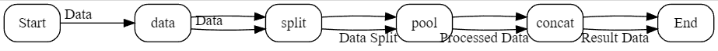
\includegraphics[width=\linewidth]{fig1.png}}
    \caption{Parallel Processing Using a Pool of Processes.}
    \label{fig1}
\end{figure}

\subsection{Model Training}
\subsubsection{XGBoost Classifier Selection}
The XGBClassifier from the XGBoost library is chosen for its robust performance and scalability. XGBoost is known for its efficiency and accuracy in handling structured data, making it suitable for our classification task.

\subsubsection{Training Data Preparation}
The extracted feature vectors and file sizes are combined to form the training dataset. Corresponding labels for each malware family are appended to create the final input for the classifier.

\begin{figure}[h]
    \centerline{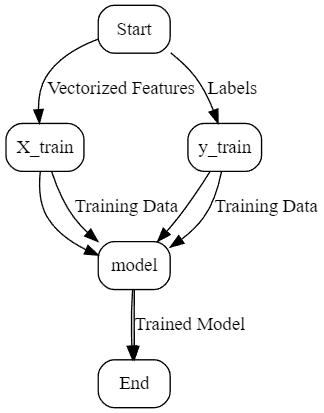
\includegraphics[width=0.4\linewidth]{fig2.png}}
    \caption{Process of Training an XGBoost Classifier.}
    \label{fig2}
\end{figure}

\begin{figure}[H]
    \centerline{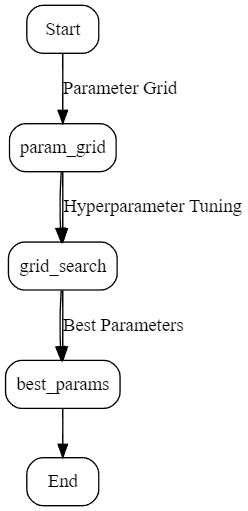
\includegraphics[width=0.4\linewidth]{fig3.png}}
    \caption{Grid Search for Hyperparameter Tuning.}
    \label{fig3}
\end{figure}

\subsubsection{Hyperparameter Tuning}
Hyperparameter tuning is performed using GridSearchCV to optimize the model's performance. Parameters such as learning rate, maximum depth, and the number of estimators are fine-tuned through cross-validation.




\subsubsection{Model Training}
The XGBClassifier is trained on the prepared training dataset using the optimized hyperparameters.

model = XGBClassifier(**best\_params)

model.fit(X\_train, y\_train)


\subsection{Model Evaluation}

\subsubsection{Cross-Validation}
Cross-validation is employed to evaluate the model’s performance. The dataset is divided into training and validation sets multiple times to ensure the model’s robustness and generalizability.

\begin{figure}[H]
    \centerline{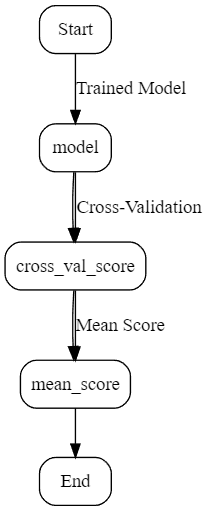
\includegraphics[width=0.35\linewidth]{fig4.png}}
    \caption{Cross-Validation for Model Evaluation.}
    \label{fig4}
\end{figure}

\subsubsection{Performance Metrics}
The model's accuracy, precision, recall, and F1-score are calculated to provide a comprehensive evaluation of its performance. These metrics assess the model's effectiveness in correctly classifying malware samples.


\subsubsection{Comparison with Baseline Models}
The performance of the XGBClassifier is compared with baseline models such as logistic regression and random forest. This comparison demonstrates the superiority of XGBoost in handling the malware classification task.

This methodology outlines a systematic approach to malware classification, from preprocessing and feature extraction to parallel processing and model training. By combining traditional machine learning techniques with advanced computational strategies, the authors provide a robust and scalable solution for large-scale malware detection and classification.

\section{Results And Discussion}


The problem at hand involves a dataset of known malware files contained within train.7z and test.7z zip files, encompassing nine different malware families. The class labels for these malware files are provided in a separate trainLabels.csv CSV file. Each malware file in the training and test sets is uniquely identified by a 20-character hash value serving as the file name, and each file belongs to a specific malware family denoted by an integer class label. The malware families included in the dataset are Ramnit, Lollipop, Kelihos\_ver3, Vundo, Simda, Tracur, Kelihos\_ver1, Obfuscator.ACY, and Gatak.

Each file's raw data contains the hexadecimal representation of the binary content, with the PE header excluded to ensure sterility. Additionally, a metadata manifest (files with a .asm extension) is provided, containing various metadata information extracted from the binary, such as function calls and strings, generated using the IDA disassembler tool.

To classify files into malware families, the following steps are taken

\begin{itemize}
    \item Equal samples are randomly selected from each class, except Simda.
    \item Hexadecimal strings (length 2) are extracted from .bytes files.
    \item A Bag-of-Words model is constructed using CountVectorizer from scikit-learn.
    \item A classification model is built using XGBClassifier from XGBoost.
\end{itemize}

The objectives of this solution are to select a balanced sample from the original dataset and improve the solution's efficiency by parallelizing computationally intensive tasks and file operations, given the substantial size of the dataset.

The project structure is meticulously organized to streamline the handling, preprocessing, and analysis of the malware classification dataset. The main directories and files are as follows

The \texttt{code/} directory contains
\begin{itemize}
    \item Microsoft Malware Classification (with Multiprocessing).ipynb: This Jupyter notebook holds the main code for the project.
    \item HexVectorizer.py: A Python script for the custom HexVectorizer used in feature extraction.
    \item Submission.csv: The final submission file containing the classification results.
\end{itemize}

The \texttt{input/} directory contains:
\begin{itemize}
    \item malware-classification/:
        \begin{itemize}
            \item trainLabels.csv: The CSV file with class labels for the training dataset.
            \item train/: This folder contains multiple .bytes files, each representing the hexadecimal content of a malware sample, such as \texttt{0ACDbR5M3ZhBJajygTuf.bytes}.
            \item test/: This folder includes multiple .bytes files for the test set, such as \texttt{ITSUPtCmh7WdJcsYDwQ5.bytes}.
        \end{itemize}
\end{itemize}

The Microsoft-malware-sample/ directory includes:
\begin{itemize}
    \item trainLabels\_bal.csv: The CSV file with balanced class labels for the training dataset.
    \item The file containing the vectorized training dataset.
    \item test\_vec.csv: The file containing the vectorized test dataset.
\end{itemize}

\subsection{Balanced Subset from Original Dataset}

\begin{figure}[h]
    \centerline{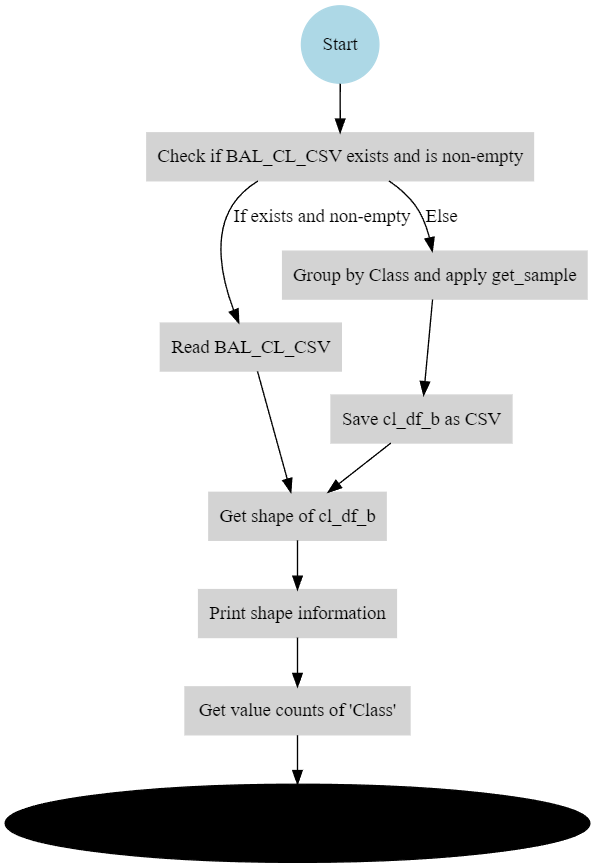
\includegraphics[width=0.7\linewidth]{fig6}}
    \caption{Workflow for Checking, Loading, and Processing Balanced Malware Subset Data.}
    \label{fig6}
\end{figure}

\begin{figure}[H]
    \centerline{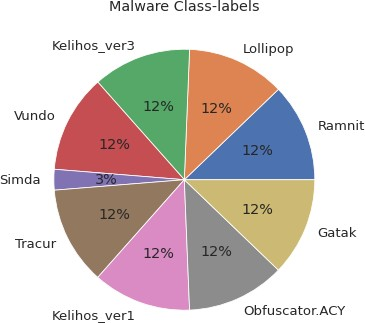
\includegraphics[width=0.7\linewidth]{fig7}}
    \caption{Malware Class-levels.}
    \label{fig7}
\end{figure}


\subsection{High Dimensional Data Visualization}

\begin{figure}[H]
    \centerline{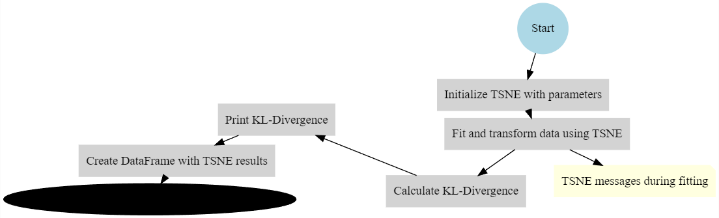
\includegraphics[width=0.7\linewidth]{fig8}}
    \caption{Workflow for TSNE Transformation and Visualization of Malware Data.}
    \label{fig8}
\end{figure}

\begin{figure}[H]
    \centerline{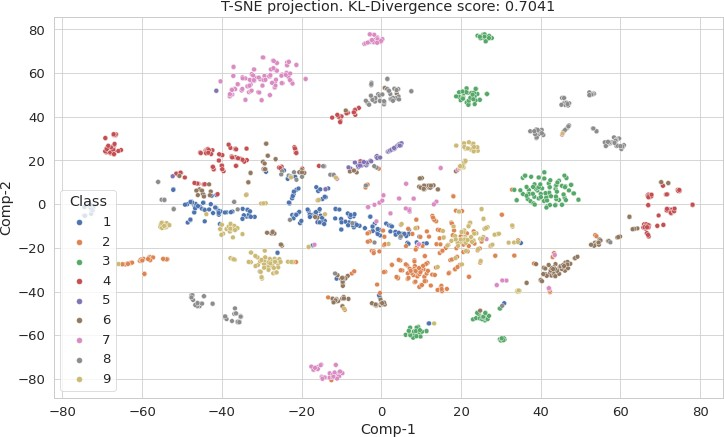
\includegraphics[width=0.7\linewidth]{fig9}}
    \caption{High Dimensional Data Visualization.}
    \label{fig9}
\end{figure}

\subsection{Tuning}
To determine the optimal range for the hyperparameters mentioned above, plot the training and validation (or test) errors. Then, identify the optimal point where:

\begin{itemize}
    \item The validation error is minimized.
    \item The gap between the training error and the validation error is smallest.
\end{itemize}

\subsubsection{Param: n\_estimators}
hyperparameter\_tuning(n\_estimators=range(1,  70,  10))

\begin{figure}[H]
    \centerline{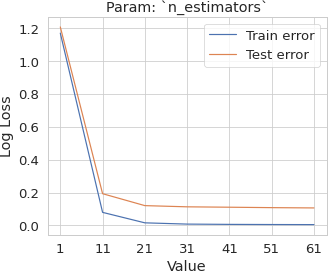
\includegraphics[width=0.7\linewidth]{fig10}}
    \caption{Param: n\_estimators.}
    \label{fig10}
\end{figure}

\subsubsection{Param: max\_depth}
hyperparameter\_tuning(n\_estimators=40,

max\_depth=range(1,  10))

\begin{figure}[H]
    \centerline{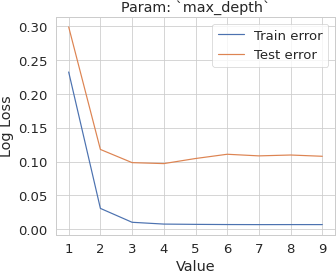
\includegraphics[width=0.7\linewidth]{fig11}}
    \caption{Param: max\_depth.}
    \label{fig11}
\end{figure}

\subsubsection{Param: learning\_rate}
\begin{figure}[H]
    \centerline{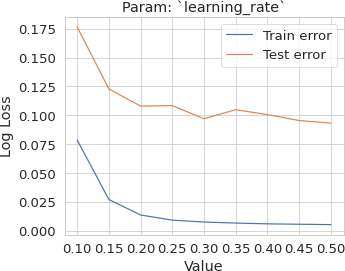
\includegraphics[width=0.7\linewidth]{fig12}}
    \caption{Param: learning\_rate.}
    \label{fig12}
\end{figure}

\subsubsection{Param: reg\_alpha}
\begin{figure}[H]
    \centerline{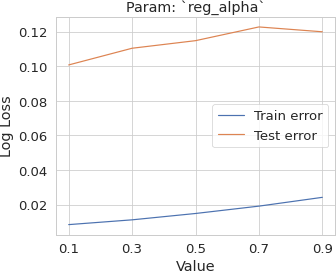
\includegraphics[width=0.7\linewidth]{fig13}}
    \caption{Param: Param: reg\_alpha.}
    \label{fig13}
\end{figure}

\subsubsection{Param: reg\_lambda}
\begin{figure}[H]
    \centerline{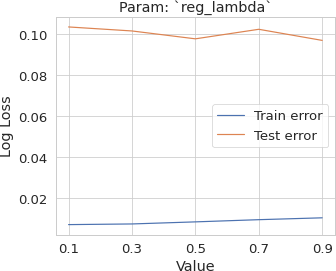
\includegraphics[width=0.7\linewidth]{fig14}}
    \caption{Param: Param: reg\_lambda.}
    \label{fig14}
\end{figure}

The project involves classifying malware files into their respective families using a combination of feature extraction, hyperparameter tuning, and model evaluation. 

\begin{itemize}
    \item \textbf{Grid Search CV}
    The model employs Grid Search CV with the XGBClassifier to fine-tune parameters. The best parameters identified are a learning rate of 0.4, max depth of 4, and 45 estimators, achieving an accuracy of 0.9604.
    \item \textbf{Model Testing}
    Feature engineering is performed by loading the vectorized test dataset or generating feature vectors from byte files. The test dataset is vectorized and saved for future use.
    \begin{figure}[H]
        \centerline{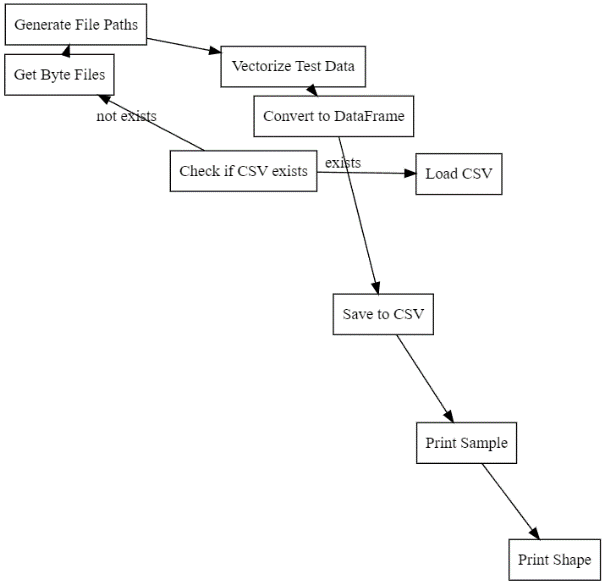
\includegraphics[width=\linewidth]{fig15}}
        \caption{Steps of the Feature Engineering Process for the Test Dataset.}
        \label{fig15}
    \end{figure}

    \item \textbf{Predictions}
    In the final step, the authors generate predictions using the trained model and save the results. Here's the process:
    \begin{itemize}
        \item Generate Predictions
        \item Prepare the Output Data
        \item Save the Predictions to CSV
    \end{itemize}
\end{itemize}
\begin{figure}[H]
    \centerline{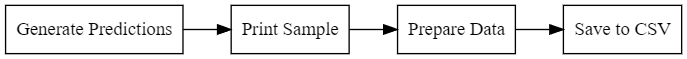
\includegraphics[width=\linewidth]{fig16}}
    \caption{The Steps Involved in Generating and Saving the Predictions.}
    \label{fig16}
\end{figure}

\section{Conclusion}
In this paper, the authors have presented a comprehensive approach to classifying malware into nine distinct families using hexadecimal representations of malware files. The methodology encompasses crucial steps in data preprocessing, feature engineering, model building, evaluation, and prediction. Firstly, the authors addressed the challenge of imbalanced data by extracting balanced samples of malware files and converting hexadecimal strings from .bytes files into numerical formats suitable for machine learning. This preprocessing step ensured a more representative dataset for training our classification model. 
Next, the authors employed feature engineering techniques, specifically building a Bag-of-Words model using scikit-learn's CountVectorizer. Utilizing precomputed vectorized datasets further streamlined our workflow, enhancing efficiency in handling large-scale data. For model building, the authors implemented an XGBoost classifier (XGBClassifier) and fine-tuned its hyperparameters using Grid Search with Cross-Validation. This optimization process aimed to achieve the best possible performance of our model in classifying malware samples into their respective families.
To evaluate the effectiveness of our model, the authors utilized cross-validation techniques and employed t-SNE visualization to gain insights into data distribution and the model's performance. Finally, predictions were generated on the test dataset and saved for submission, completing the classification process. Through the use of parallel processing and efficient data handling techniques, the authors significantly reduced computation time without compromising on accuracy. Overall, this study outlines a robust mechanism for malware classification that can be further enhanced with additional metadata and advanced feature engineering techniques. 


\begin{thebibliography}{00}
\bibitem{b1} Yoshikawa, Yuya, Tomoharu Iwata, and Hiroshi Sawada. "Latent Support Measure Machines for Bag-of-Words Data Classification." Proceedings Article, 2014.
\bibitem{b2} Ronghui, Zihan Zhang, Ziye Wang, Suyang Dai, Hiroshi Mamitsuka, and Shanfeng Zhu. "AttentionXML: Label Tree-based Attention-Aware Deep Model for High-Performance Extreme Multi-Label Text Classification." Proceedings Article, 2019.
\bibitem{b3} Banerjee, Shobhan, Bibhuti Bhusan Dash, M. Rath, Tanmaya Swain, and Tapaswini Samant. "Malware Classification using Bigram BOW, Pixel Intensity Features, and Multiprocessing." Proceedings Article, 2022. doi: 10.1109/CONECCT55679.2022.9865764.
\bibitem{b4} Chen, Zhiguo, and Xuanyu Ren. "An Efficient Boosting-Based Windows Malware Family Classification System Using Multi-Features Fusion." Journal Article, Applied Sciences, 2023. doi: 10.3390/app13064060.
\bibitem{b5} Onoja, M. Nelson, Abayomi Jegede, N.V Blamah, Abinbola Victor Olawale, and Temidayo Oluwatosin Omotehinwa. "EEMDS: Efficient and Effective Malware Detection System with Hybrid Model based on XceptionCNN and LightGBM Algorithm." Journal Article, 2022.
\end{thebibliography}


\end{document}
